% !TeX root=../main.tex

\subsection{Alignment Strategy}\label{subsec:as}
When aligning a log trace with a TG, retrieving the model trace maximizing the combined provision of minimum trace alignment cost 
and maximum model trace probability does not suffice.
Hence, we find the best $k$ alignments among all the distinct \unravelled\ model traces in $\ptraces{\tg}{\pmin}$. This is
known as the $k$-nearest neighbors ($k$NN) problem of finding the $k$ nearest data points to a \textit{query} $x$ from a set 
$\mathcal{X}$ of \textit{data points} w.r.t.\ a given distance function $d_k$. Through ad-hoc data structures, such as VP-Trees 
and KD-Trees, %VP-Trees \cite{Fu2000} \cite{Maneewongvatana99}, and M-Trees \cite{Ciaccia},
we can retrieve the $k$-neighborhood of $x$ in $\mathcal{X}$ by pre-ordering (\textit{indexing}) $\mathcal{X}$ w.r.t.\ $d_k$ 
and searching from the top-$1$ alignment.
%
To align a trace $\logtrace$ over the \unravelled\ traces $\ptraces{\tg}{\pmin}$,
the $k$-Nearest Neighbors describe the best $k$ alignments for $\logtrace$. We discuss two strategies to obtain these
alignments.

\noindent
\textbf{Optimal-Ranking Trace Aligner.}
One approach is to reuse existing trace aligners; e.g., \cite{DBLP:conf/edoc/AdriansyahDA11,LeoniM17} over the Levenshtein 
distance.
Using decision theory \cite{dectheor}, we express the ranking score as the product 
$\probskip{\nonlogtrace} d(\logtrace,\nonlogtrace)$, taking into account the cost of the alignment (the distance between 
the model trace and the trace to be aligned) and the probability of the model trace.

To represent the same intuition of a weighted distance as a ranking function, we transform it into a
similarity function returning $1$ when $\nonlogtrace=\logtrace$ and $\probskip{\logtrace}=1$ hold. We express $d$ as
a normalized similarity score $s_d(\logtrace,\nonlogtrace):=\frac{1}{\frac{1}{c}d(\logtrace,\nonlogtrace)+1}$, where  
$c\in\mathbb{N}_{\neq0}$ is a constant. The maximum similarity is reached when the distance is $0$ and the similarity decreases 
as the distance increases. 
 The golden ranking function producing the optimal ranking is 
 $\goldenrank(\logtrace,\nonlogtrace)=\probskip{\nonlogtrace} \probskip{\logtrace} s_d(\logtrace,\nonlogtrace)$;
${\max\arg}_{\nonlogtrace\in \WCal{\pmin}{n}} \goldenrank(\logtrace,{\nonlogtrace})$ yields the best optimal-ranking trace 
alignment for a log trace $\logtrace$, where $\goldenrank$ must be computed anew for each possible $\logtrace$. 
{We can represent each trace as a point  $(\mathbb{P}_N(\sigma)\mathbb{P}_N(\sigma'),\; s_d(\sigma,\sigma'))$ in the 
2-dimensional similarity/probability space of coordinates $(p,s)$, reducing the trace finding problem to maximising the product 
$p\cdot s\equiv \mathbb{P}_N(\sigma)\mathbb{P}_N(\sigma')\cdot s_d(\sigma,\sigma')$ (Figure \ref{fig:sps}).}
%
\begin{figure}[!t]
	\centering
	\subfloat{\label{fig:spp}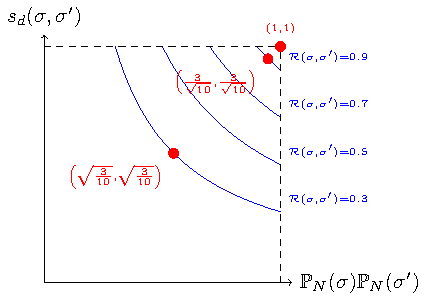
\includegraphics[width=.35\textwidth]{images/original_space.pdf}}\qquad
	\subfloat{\label{fig:knnspace}\includegraphics[width=.33\textwidth]{images/transformed_space.pdf}}\\
	\caption{Two characterizations of probabilistic trace alignment; the similarity/probability space above, and the transformed
	$k$NN space below. The best possible match is shown in red in both spaces.}\label{fig:sps}
\end{figure}


\begin{table}[!t]
\centering
\caption{Golden ranking of $\ptraces{\closed{\tg}}{0}$ with maximum length $4$, where $\logtrace=\const{caba}$ and $c=5$.}\label{tab:expected}
\resizebox{.45\textwidth}{!}{\begin{tabular}{lc|ll|c}
	\toprule
	
	{$\nonlogtrace$} &
	{$d(\sigma',\sigma)$} &
	$( \mathbb{P}_N(\sigma')$ &  $,\,s_d(\sigma',\sigma)) $ &
	{$\approx s_d(\sigma,\sigma^*)\cdot w_\sigma$} \\
	
	
	\midrule
	$\const{a}$  & $3$ & $0.4$ & $\;\; 0.6250$  & $0.2500$\\
	$\const{aa}$  & $2$ & $0.2$ & $\;\; 0.7142$ & $0.1428$\\
	$\const{aaa}$  & $2$ & $0.1$ & $\;\; 0.7142$ & $0.0714$ \\
	$\const{ca}$  & $2$ & $0.07$ & $\;\; 0.7142$ & $0.0500$\\
	$\const{cb}$  & $2$ & $0.06$ & $\;\; 0.7142$ & $0.0428$ \\
	$\const{aaaa}$  & $3$ & $0.05$ & $\;\; 0.7142$ & $0.0357$ \\
	$\const{caa}$  & $1$ & $0.035$ & $\;\; 0.8333$ & $0.0292$ \\
	$\const{caaa}$  & $1$  & $0.0175$ & $\;\; 0.8333$ & $0.0145$ \\
	\bottomrule
\end{tabular}}
\end{table}
\begin{example}\label{ex:rankingTaus}
Consider the TG $\closed{\tg}$ in \figurename~\ref{fig:lmc} with probabilities
$\pa=0.8$, $\pb=0.2$, $\pc=\pf=0.5$, $\pd=0.7$, and $\pe=0.3$. The traces with maximum length $4$ are:
%$$\begin{aligned}
%\ptraces{\expN}{0}_{|\nonlogtrace|\leq 4}=
$\{\braket{\const{a},0.4},\braket{\const{aa},0.2}$, $\braket{\const{aaa},0.1}$, $\braket{\const{ca},0.07}$, 
$\braket{\const{cb},0.06}$,
$\braket{\const{aaaa},0.05},\braket{\const{caa},0.035},\braket{\const{caaa},0.0175}\}$. 
Table \ref{tab:expected} represents their alignment raking with  $\nonlogtrace=\textup{caba}$.  Although $\const{caa}$ and 
$\const{caaa}$ are the most similar to $\const{caba}$, their associated probability  is rather low, so traces with 
higher probability but lower similarity score are preferred (e.g., $\const{a}$ and $\const{aa}$).
\end{example}
%
{Since users might still prefer the most similar ones to the ones maximizing both probability and similarity, we 
return the best $k$ solutions.
We reduce the problem to $k$NN over the Euclidean Space through a transformation $t$ such that the distance of the 
transformed point $t(p,s)$ from  the origin $\vec{0}$ is $\sfrac{1}{ps}$. This preserves the score from the golden ranking 
and maps the points maximizing $ps$ nearer to the origin. We choose}
$t(p,s):=\left(\frac{1}{s\sqrt{p^2+s^2}},\; \frac{1}{p\sqrt{p^2+s^2}}\right)$. 
Our search always starts from the origin, and hence finds the best candidates first.
	
%
\begin{example}
{Figure \ref{fig:sps} (above) shows a family of hyperbolae $ps$ with all the alignments having 
$\mathcal{R}(\sigma,\sigma')=ps$. Point $\color{red}(1,1)$ is the best possible trace match, i.e., a trace 
$\nonlogtrace\in\ptraces{G}{0}$ with $\nonlogtrace=\logtrace$ and $\mathbb{P}_G(\nonlogtrace)\mathbb{P}_G(\logtrace)=1$.
%		
Figure \ref{fig:knnspace} (below) shows that the embedding moves the points of the hyperbola $ps$ to a circumference $x^2+y^2=\sfrac{1}{(ps)^2}$ describing a locus of the points equidistant as $\sfrac{1}{ps}$ from the origin of the axes $(0,0)$.}
\end{example}
%
The transformation required for running the $k$NN algorithm preserves the ranking induced by $\mathcal{R}$.

\begin{lemma}
The set of points having the product $ps$ at least $k\in[0,1]$ corresponds to the set of $t$-transformed points with distance 
at least $1/k$ from the origin.
\end{lemma}
%
\begin{proof} 
\todo{may be removed if needed}
Ignoring the irrelevant traces for $ps= 0$, we have:
	\[
	ps\geq k\Leftrightarrow \frac{1}{ps}=
	{ \frac{\sqrt{p^2+s^2}}{ps\sqrt{p^2+s^2}}= \left\|t(p,s)-\vec{0}\right\|_2\leq\frac{1}{k} }\\
	%&{\Leftrightarrow \sqrt{\frac{p^2+s^2}{p^2s^2(p^2+s^2)}}\leq\frac{1}{k}} \\
%	&{\Leftrightarrow \sqrt{\frac{p^2}{p^2s^2(p^2+s^2)}+\frac{s^2}{p^2s^2(p^2+s^2)}}\leq\frac{1}{k}} \\
%	&{\Leftrightarrow \sqrt{\frac{1}{s^2(p^2+s^2)}+\frac{1}{p^2(p^2+s^2)}}\leq\frac{1}{k}} \\
%	&{\Leftrightarrow \left\|{\biggr({\frac{1}{s\sqrt{p^2+s^2}},\frac{1}{p\sqrt{p^2+s^2}}\biggr)}-\vec{0}}\right\|_2\leq\frac{1}{k}} \\
\]
\end{proof}
	
\noindent
\textbf{Approximate-Ranking Trace Embedder.}\label{subsec:ate}
Ranking optimality comes at the cost of a brute-force recomputation of $\goldenrank$ for each trace $\logtrace$ to align.
Since each embedding $\phi$ entails an associated similarity metric $k_\phi$ (\S\ref{subsec:katk}) and hence an associated
distance $d_{k_\phi}$ (Equation \ref{eq:dofk}), we can compute the embeddings for all the \unravelled\ traces
before the top-$k$ search ensuring that they are independent of the trace to align, avoiding the brute-force cost. 
This computational gain comes with a loss in precision; the generation of precise embeddings for graph data with loops is 
NP-complete \cite{GartnerFW03} and, in its approximated version, is unable to accurately represent data using low-dimensional 
vectors \cite{Seshadhri5631}. Our proposed embedding ($\gorgembed$) is thus weakly-ideal (\S\ref{subsec:katk}).

$\gorgembed$ is a variant of the embedding $\trembed$ from \cite{LodhiSSCW02}, which addresses some of its shortcomings.
Indeed, $\trembed$
\begin{alphalist}
 \item is not weakly-ideal, so we cannot numerically assess if two embeddings represent equivalent traces 
 (Example \ref{ex:wheredotiszero});
 \item does not characterize $\tau$-moves, so the probabilities of the initial and final $\tau$-moves are not preserved; and
 \item is affected by numerical errors from finite arithmetics: longer traces $\nonlogtrace$ generated from skewed probability 
 	distributions $G.\Lambda^i$ yield greater truncation errors, as smaller $\lambda^i$ components for bigger 
 	$i<|\nonlogtrace|$ are ignored, preventing a complete numerical vector characterization of  $\nonlogtrace$ in practice.
\end{alphalist}
%
To overcome these shortcomings we 
\begin{alphalist} 
\item propose a weakly-ideal embedding, which also 
\item exploits an $\omega$ factor for preserving probabilities from and to $\tau$ transitions, and 
\item mitigate the numerical truncation errors induced by trace length and probability distribution skewness through two 
sub-embedding strategies, $\epsilon^x$ and $\nu^x$. The former descends from $\trembed$ and the latter approximates 
the trace similarity through label frequencies.
\end{alphalist}

Since a trace embedding for $\nonlogtrace$ representing the transitions in $\closed{\tg}.\Lambda$ requires an intermediate 
TG representation, each $\nonlogtrace$ is mapped to a transition graph $\tg_\nonlogtrace$.
%
\begin{definition}[trace projection]
Let $\closed{G}=(V,s,t,L,R)$ be a $\tau$-closed TG, and $\pmin\in(0,1]$. The $\closed{G}$ \emph{projection} over the trace 
$\nonlogtrace$ is the weighted TG $(\closed{G}_\nonlogtrace,\omega)$, where $\closed{G}_\nonlogtrace$ is the TG 
$(V_\nonlogtrace,s,t,L_\nonlogtrace,R_\nonlogtrace)$ where
$V_\nonlogtrace$ contains the nodes generating $\nonlogtrace$ from $\closed{G}$	
	(i.e., $\bigcup_{\xi\in\runs{\nonlogtrace}{\closed{G}}}\seqs{\xi}{ \closed{G}}$) and
$L_\nonlogtrace$ and $R_\nonlogtrace$ are the restrictions of $L$ and $R$ to $V_\nonlogtrace$; and
$$\omega := 1-\prod_{\xi\in\runs{\sigma}{\closed{G}},\eta\in\seqs{\xi}{\closed{G}}}\Big(1-(\textit{ifte}([L]_{\tau\eta_1},[R]_{\eta_1\eta_2})\textit{ifte}([L]_{\tau t_n},[R]_{t_{n-1} t_n})\Big),$$
	where $\textit{ifte}(x,y):=x(y-1)+1$ returns $y$ if $x=1$ and $1$ otherwise. We denote the set of all the $\closed{G}_\nonlogtrace$ as $\TBf{\pmin}{4}(\closed{G})$.\todo{need to understand this}
%\dots
%		
%		\dots we generate a set $\TBf{\pmin}{n}(\closed{G})$ of projected TGs $P$ for each trace in $\WCal{\pmin}{n}(P)$ as follows: for each weighted trace $\braket{\nonlogtrace,\probskip{\nonlogtrace}}\in\WCal{\pmin}{n}(P)$ generated from a path $\pi_\nonlogtrace=s\to n_2\rightsquigarrow n_m\to t$ over $R$, we generate a TG $P_\nonlogtrace=(s',t',L_\nonlogtrace,R_\nonlogtrace,\omega')$, where \begin{inparaenum}[\it (i)]
%			\item $s'=s$ if $\textit{label}(s)\neq \tau$ and $t'=n_2$ otherwise,
%			\item $t'=t$ if $\textit{label}(t)\neq \tau$ and $t'=n_m$ otherwise,
%			\item $L_\nonlogtrace$ (and $R_\nonlogtrace$) is the submatrix of $L$ (and $R$) over the non-$\tau$ labeled notes in $\pi_\nonlogtrace$ and the labels from $\nonlogtrace$,
%			\item $\omega'$ is initialized by $\omega$ and then multiplied by $[R]_{s,n_2}$ (and also $[R]_{n_m,t}$) if $\textit{label}(s)=\tau$ (and  $\textit{label}(t)=\tau$).
%		\end{inparaenum}
\end{definition}
%	
\begin{table}[!t]
	\caption{Projections of $\tg$ over traces of length $4$.}\label{tab:proj}
	\centering
	\resizebox{.28\textwidth}{!}{\begin{tabular}{>{\centering\arraybackslash} m{1cm}| >{\centering\arraybackslash} m{4cm} >{\centering\arraybackslash} m{1cm} >{\centering\arraybackslash} m{1cm} }
			\toprule
			$\nonlogtrace$&$G_\nonlogtrace$&$l$&$\omega$\\
			\midrule
			$\const{a}$ & \includegraphics{images/trace_a} & $1$ & $\color{violet}\pa\pf$\\
			$\const{cb}$ & \includegraphics{images/trace_cb} & $2$ & $\color{violet}\pb$\\
			$\const{aaa}$ & \includegraphics{images/trace_a_loop} & $3$ & $\color{violet}\pa\pf$\\
			$\const{caa}$ & \includegraphics{images/trace_caa} & $3$ & $\color{violet}\pb\pf$\\
%			\bottomrule
%	\end{tabular}}\qquad 	
%	\resizebox{.3\textwidth}{!}{\begin{tabular}{>{\centering\arraybackslash} m{1cm}| >{\centering\arraybackslash} m{4cm} >{\centering\arraybackslash} m{1cm} >{\centering\arraybackslash} m{1cm} }
%	\toprule
%	$\nonlogtrace$&$G_\nonlogtrace$&$l$&$\omega$\\
%	\midrule
	$\const{aa}$ & \includegraphics{images/trace_aa} & $2$ & $\color{violet}\pa\pf$\\
	$\const{ca}$ & \includegraphics{images/trace_ca} & $2$ & $\color{violet}\pb\pf$\\
	\begin{tabular}{l}aaaa\end{tabular} & \includegraphics{images/trace_a_loop} & $4$ & $\color{violet}\pa\pf$\\
	$\const{caaa}$ & \includegraphics{images/trace_ca_loop} & $4$ & $\color{violet}\pb\pf$\\
	\bottomrule
\end{tabular}}
\vspace{-0.2cm}
\end{table}
The graph weight $\omega$ derives from the outgoing edges of the initial node and the ingoing edges of the accepting node; 
such nodes are labeled as $\tau$. Since the embedding strategy from \cite{LodhiSSCW02} considers only visible 
transitions, and the trace extraction process discards the $\tau$ information, we use $\omega$ to preserve such information.
%
\begin{example}\label{ex:neue}
Table \ref{tab:proj} shows the projected TGs from the traces from Example \ref{ex:rankingTaus}, where only the relevant 
embedding information is displayed (e.g., $\tau$-labeled nodes are removed).
\end{example}
%	
The embedding $\gorgembed$ is computed for each TG generated by projections. The goal is to use
$k_{\gorgembed}$ for ranking the traces generated by \unravelling\ such graphs. We extend the embedding from 
\cite{LodhiSSCW02} by including the associated probability, and making the ranking induced by $k_{\gorgembed}$ the inverse of 
that induced by the
sum of the following distances: the transition correlations $\epsilon$ and the transition label frequency $\nu$.
%\xout{Given that we previously observed that a TGs $\closed{\tg_{\rg{\net}}}$ can be fully characterized (read, similarity) by their associated set of traces $\mathcal{W}_p^n(P)$  and that the trace embedding can be described as an embedding over a TG, we can characterize a TG embedding as a transition matrix embedding. In addition to that, when two Workflow Nets share similar node labelings but no ${\color{green}\alpha}\rightsquigarrow{\color{green}\beta}$ paths for any ${\color{green}\alpha}$ and ${\color{green}\beta}$, we should combine the former embedding with an embedding characterizing the frequency on how the nodes' labels appear in the generated traces.} \ADD

We require that the desired properties of $\gorgembed$ are independent of the characterization of $\epsilon$ over the 
$2$-grams in $\tasks^2$ and $\nu$ over the labels in $\tasks$, which  provide different embedding strategies.  Thus, our embedding is defined for any weighted TG.



%\begin{table}[!t]
%	\centering
%	\caption{Embedding representation for the TG $P$ in \figurename~\ref{fig:closed} and the trace $\logtrace=\textup{caba}$ after representing it as in \figurename~\ref{fig:sigmastar}. Please note that we restrict $\trace_\tau^2$ to the one from $P$.}\label{tab:emb1}
%		\begin{tabular}{l|l|l|l|l|l|l|}
%	\toprule
%	& a    & b                                                   & c    & aa   & ca   & cb   \\
%	\midrule
%	$\gorgembed(P)$ & $9.94\cdot10^{-25}$ & $1.18\cdot 10^{-26}$ & $1.04\cdot10^{-25}$ & $4.45\cdot 10^{-25}$ & $6.22\cdot10^{-25}$ & $8.29\cdot10^{-26}$\\
%	$\gorgembed(P_{\logtrace})$ & $8.16\cdot10^{-17}$ & $4.08\cdot 10^{-17}$ & $4.08\cdot10^{-17}$ & $4.37\cdot 10^{-17}$ & $1.03\cdot10^{-16}$ & $4.37\cdot10^{-17}$\\
%	\bottomrule
%\end{tabular}
%\end{table}
\begin{definition}[G-Embedding]\label{def:ppne}
Given a weighted TG $(G,\omega)$ with $G=(V,s,t,L,R)$ and a tuning parameter $t_f\in[0,1]$, the \emph{G-Embedding} 
$\gorgembed$ over the visible $2$-grams and transition labels, $\tasks\cup\tasks^2$, is defined by
$$\gorgembed_{i}(G)=\begin{cases}
	\omega \frac{\epsilon_\const{ab}(G)}{\|\epsilon\|_2}\;t_f^{|R>0|}\, & {i}=\const{ab}\in\tasks^2\\
	\frac{\nu_\const{a}(G)}{\|\nu\|_2}\;\;\;\,t_f^{|R>0|}\, & {i}=\const{a}\in\tasks\\
\end{cases}$$
%<<<<<<< HEAD
%where $\nu$ (and $\epsilon$) represents the non-negatively defined embeddings associated to $G.L$ (both $G.R$ and $G.L$): {we require that  $\epsilon$  returns $\epsilon_\const{ab}=0$ for the $2$-grams $\const{ab}$ that are not represented within the Transition Graph ($\forall \const{ab}\in\tasks^2.\; \left(\forall i\in\mathbb{N}_{\neq0}. [LR^iL^t]_\const{ab}=0\right) \Leftrightarrow \epsilon_\const{ab}(G)=0$), and either $\nu$ always returns the empty vector or $\nu_\const{a}(G)=0$ iff. the labels $\const{a}\in\tasks$ that are associated to no vertex in $V$ ($\forall \const{a}\in\tasks. \left(\forall u\in V. L_{\const{a}u}=0\right)\Rightarrow \nu_\const{a}(G)=0$).}
%=======
where $\nu$ (and $\epsilon$) represents the non-negatively defined embeddings associated to $G.L$ (both $G.R$ and $G.L$): 
\ADD{$\epsilon$ returns $\epsilon_\const{ab}=0$ for the $2$-grams $\const{ab}$ that are not represented within the TG 
and either $\nu$ always returns the empty vector or $\nu_\const{a}(G)=0$ iff the labels $\const{a}\in\tasks$ that are associated to no vertex in $V$} % ($\forall \const{a}\in\tasks. \left(\forall u\in V. L_{\const{a}u}=0\right)\Rightarrow \nu_\const{a}(G)=0$).}
%>>>>>>> 5033e447c99df01a59a65a68a0b9dca3febeaa15
\end{definition}
%
Here, ${\max\arg}_{\nonlogtrace\in \WCal{\pmin}{n}, G_\nonlogtrace\in\TBf{p}{n}(P)} k_{\gorgembed}(G_\logtrace, G_{\nonlogtrace})$ returns the best approximated trace alignment for a log trace represented as $G_{\logtrace}$. %\xout{Similarly, we can provide the TG $P\in\mathbf{P}$ providing the best approximated alignment for $P_{\logtrace}$ as $\underset{P}{\max\arg}\underset{ P_\trace\in\mathbf{P}_p^n(P)}{\max} k_{\gorgembed}(P_\trace, P_{\logtrace})$.}¯
%
\begin{table}[!t]
	\caption{Different sub-embeddings ($\epsilon^1$, $\epsilon^2$, $\nu^1$, and $\nu^2$) for $\gorgembed$.}\label{tab:embedstrat}
	\centering
	\resizebox{.45\textwidth}{!}{\begin{tabular}{c|c|c}
		\toprule
		& $x=1$ & $x=2$ \\
		\midrule
		$\epsilon^x_\const{ab}(G):=$ & $\label{eq:epsilon}
		\sum_{i=1}^l{\lambda^i}\frac{[LR^iL^t]_\const{ab}}{\sum_{\const{a'b'}\in\tasks^2}R^i_\const{a'b'}}$ & $
		\sum_{i=1}^l\lambda^i[\Lambda^i]_\const{ab}$\\
		$\nu^x_\const{a}(G):=$ & $\frac{1}{c}\sum_{\nonlogtrace'\in \ptraces{G}{0}}\frac{|\Set{\nonlogtrace_i'\in\nonlogtrace'|\const{a}\in\tasks\wedge \nonlogtrace'_i=\const{a}}|}{|\nonlogtrace'|}$ & $0$ \\
		\bottomrule
	\end{tabular}}
\end{table}
%
For sub-embeddings $\epsilon$ and $\nu$, {in our experiment section}, we choose two possible interchangeable definitions ($x=1$ and $x=2$) shown in Table \ref{tab:embedstrat}: here, $l$ is the path length (reported in Table \ref{tab:proj}), and $c$ for $\nu^1$ is a normalization factor such that $\sum_{\const{a}\in\tasks}\nu^1_\const{a}(P)=1$. While $\nu^2$ implies to completely ignore the label frequency contribution, $\epsilon^2$ is the direct implementation of $\trembed$ from \S\ref{subsec:katk}, and $\epsilon^1$ and $\epsilon^2$ only differ from the normalization perspective. $t_f\in [0,1]\subseteq\mathbb{R}^+_{0}$ and $\lambda\in (0,1]\subset\mathbb{R}^+_{0}$ are tuning parameters that can be
inferred from the available data \cite{DriessensRG06}. The latter describes the previously mentioned decay factor, while $t_f$
represents the relevance of our embedding representation as the number of edges within $\closed{G}_\nonlogtrace$ increases. In our experiments and
examples, we choose $t_f=0.0001$ and $\lambda=0.07$.



%In Example \ref{ex:cmpexample}, we will see that the given definition of $\epsilon^1$ provides a better approximation than the edge embedding $\epsilon^2$.


This representation is independent of the representation associated with a trace to be aligned. Therefore it does not have to be recomputed at each alignment with a different $\logtrace$.



%When the transition matrix is ergodic \cite{StocasticCC},  the transition matrix embedding converges to $\epsilon(R)_{\color{green}\alpha\beta}=[(\mathbf{I}-\lambda\Lambda)^{-1}]_{\color{green}\alpha\beta}$ \cite{GartnerFW03} for $n\to+\infty$.

\begin{table*}[!t]
	\centering
	\caption{Embeddings for $\net$-traces of maximum length $4$ and $\logtrace=\const{caba}$.}\label{tab:emb2}\label{tab:embsitar}
	\resizebox{\textwidth}{!}{\begin{tabular}{lllllllllllll}
		\toprule
		& $\const{a}$    & $\const{b}$                                                   & $\const{c}$    & $\const{aa}$  & $\const{ab}$   & $\const{ac}$   & $\const{ba}$  & $\const{bb}$   & $\const{bc}$   & $\const{ca}$   & $\const{cb}$  & $\const{cc}$  \\
		\midrule		
		$\gorgembed(\overline{G}_\const{aaaa})$ & $1.00\cdot 10^{-24}$ & $0.00\cdot 10^{0}$   & $0.00\cdot 10^{0}$   & $6.44\cdot 10^{-26}$ & $0.00\cdot 10^{0}$& $0.00\cdot 10^{0}$& $0.00\cdot 10^{0}$& $0.00\cdot 10^{0}$& $0.00\cdot 10^{0}$    &$0.00\cdot 10^{0}$& $0.00\cdot 10^{0}$& $0.00\cdot 10^{0}$ \\
		$\gorgembed(\overline{G}_\const{aaa})$  & $1.00\cdot 10^{-24}$ & $0.00\cdot 10^{0}$   & $0.00\cdot 10^{0}$   & $1.29\cdot 10^{-25}$ & $0.00\cdot 10^{0}$& $0.00\cdot 10^{0}$& $0.00\cdot 10^{0}$& $0.00\cdot 10^{0}$& $0.00\cdot 10^{0}$    &$0.00\cdot 10^{0}$& $0.00\cdot 10^{0}$& $0.00\cdot 10^{0}$ \\
		$\gorgembed(\overline{G}_\const{aa})$   & $1.00\cdot 10^{-24}$ & $0.00\cdot 10^{0}$   & $0.00\cdot 10^{0}$   & $2.57\cdot 10^{-25}$ & $0.00\cdot 10^{0}$& $0.00\cdot 10^{0}$& $0.00\cdot 10^{0}$& $0.00\cdot 10^{0}$& $0.00\cdot 10^{0}$    &$0.00\cdot 10^{0}$& $0.00\cdot 10^{0}$& $0.00\cdot 10^{0}$ \\
		$\gorgembed(\overline{G}_\const{a})$    & $1.00\cdot 10^{-4}$  & $0.00\cdot 10^{0}$   & $0.00\cdot 10^{0}$   & $0.00\cdot 10^{0}$   & $0.00\cdot 10^{0}$& $0.00\cdot 10^{0}$& $0.00\cdot 10^{0}$& $0.00\cdot 10^{0}$& $0.00\cdot 10^{0}$    &$0.00\cdot 10^{0}$& $0.00\cdot 10^{0}$& $0.00\cdot 10^{0}$ \\
		$\gorgembed(\overline{G}_\const{caa})$  & $7.07\cdot 10^{-25}$ & $0.00\cdot 10^{0}$   & $7.07\cdot 10^{-25}$ & $1.46\cdot 10^{-25}$ & $0.00\cdot 10^{0}$& $0.00\cdot 10^{0}$& $0.00\cdot 10^{0}$& $0.00\cdot 10^{0}$& $0.00\cdot 10^{0}$    &$2.05\cdot 10^{-25}$& $0.00\cdot 10^{0}$& $0.00\cdot 10^{0}$ \\
		$\gorgembed(\overline{G}_\const{ca})$   & $7.07\cdot 10^{-25}$ & $0.00\cdot 10^{0}$   & $7.07\cdot 10^{-25}$ & $0.00\cdot 10^{0}$   & $0.00\cdot 10^{0}$& $0.00\cdot 10^{0}$& $0.00\cdot 10^{0}$& $0.00\cdot 10^{0}$& $0.00\cdot 10^{0}$    &$1.00\cdot 10^{-8}$& $0.00\cdot 10^{0}$& $0.00\cdot 10^{0}$ \\
		$\gorgembed(\overline{G}_\const{cb})$   & $0.00\cdot 10^{0}$   & $7.07\cdot 10^{-25}$ & $7.07\cdot 10^{-25}$ & $0.00\cdot 10^{0}$   & $0.00\cdot 10^{0}$& $0.00\cdot 10^{0}$& $0.00\cdot 10^{0}$& $0.00\cdot 10^{0}$& $0.00\cdot 10^{0}$    &$0.00\cdot 10^{0}$ & $4.29\cdot 10^{-9}$& $0.00\cdot 10^{0}$ \\
		$\gorgembed(\overline{G}_\const{caaa})$ & $7.07\cdot 10^{-25}$ & $0.00\cdot 10^{0}$   & $7.07\cdot 10^{-25}$ & $1.03\cdot 10^{-25}$ & $0.00\cdot 10^{0}$& $0.00\cdot 10^{0}$& $0.00\cdot 10^{0}$& $0.00\cdot 10^{0}$& $0.00\cdot 10^{0}$    &$7.20\cdot 10^{-26}$ & $0.00\cdot 10^{0}$& $0.00\cdot 10^{0}$ \\
		\bottomrule
				$\gorgembed(\overline{G}_\const{caba})$ & $8.16\cdot10^{-17}$ & $4.08\cdot 10^{-17}$ & $4.08\cdot10^{-17}$ & $4.37\cdot 10^{-17}$ &  $0.00\cdot 10^{0}$& $0.00\cdot 10^{0}$& $0.00\cdot 10^{0}$ & $0.00\cdot 10^{0}$ & $0.00\cdot 10^{0}$    & $1.03\cdot10^{-16}$ & $4.37\cdot10^{-17}$& $0.00\cdot 10^{0}$ \\
		\bottomrule
	\end{tabular}}

\end{table*}
\begin{example} %\small \label{ex:withpaths} %After generating all the TGs for the \unravelled\ traces (Example \ref{ex:neue}), we further associate a sub-embedding $\epsilon$ using the $2$-grams included in the model traces.\footnoteref{fn:caveat}
%Given $\nonlogtrace_\tau=\Set{a,b,c}$, the embedding space is of size $6$: three features (computed using $\nu$) correspond to the labels of the non-$\tau$ vertices in $\nonlogtrace_\tau$, i.e., $\{a,b,c\}$, and other three features (computed using $\epsilon$) correspond to the $2$-grams subsequences that are also traces in $W^4_0(P)$, i.e., $\{aa,ca,cb\}$. Therefore, $\{a,b,c,aa,ca,cb\}\subset \nonlogtrace_\tau^2\cup\nonlogtrace_\tau$ is the whole set of features describing both the label and the transition matrix, so $\gorgembed$ is a vector with 6 dimensions.
%\xout{The embedding associated to $P$ is described in Table \ref{tab:emb1} as $\gorgembed(P)$: it shows that doing ${\color{green}a}\rightsquigarrow{\color{green}a}$ is more probable than doing  ${\color{green}c}\rightsquigarrow{\color{green}a}$. Also, given that both the probability of performing ${\color{green}c}\overset{1}{\rightsquigarrow}{\color{green}b}$ is relatively low and trace $\color{green}cb$ is relatively infrequent, ${\color{green}c}{\rightsquigarrow}{\color{green}b}$ is less probable than any other subtrace. If we now consider the single nodes, $\color{green}c$ shares a subset of traces with $\color{green}a$ where $\color{green}a$ is more frequent than $\color{green}c$, and therefore the score of the former is higher than the one of the latter. Also, the score associated to the single node $\color{green}b$ is lower than the one for the single node $\color{green}c$ because $\color{green}b$ is less frequent and appears in less probable traces than $\color{green}c$: in particular, $\color{green}c$ appears in \textit{ca}, which is more probable than \textit{cb}.}
Table \ref{tab:emb2} shows the embeddings $\gorgembed(\overline{G}_\nonlogtrace)$ generated from Example \ref{ex:neue}, where the $l=|\nonlogtrace|$ for each $\unravelled$ trace $\nonlogtrace$.
{After representing trace $\logtrace=\const{caba}$ to be aligned as a graph (\figurename~\ref{fig:taustar}), we can represent its}
%\xout{Similar considerations can be also drawn from the}
embedding $\gorgembed(\overline{G}_{\logtrace})$ with strategies $\epsilon^1$ and $\nu^1$ %\xout{associated to the trace $\logtrace=\textup{caba}$ (also in Table --):} \ADD
{as} in Table \ref{tab:embsitar}: $\const{a}$ is clearly the most frequent label while $\const{b}$ and $\const{c}$ are equiprobable. The $2$-gram $\const{ca}$ appears twice in the trace set and then, it is more frequent than the remaining $2$-grams.
\end{example}

{We can also prove that such sub-embeddings satisfy the conditions required by the G-Embedding. }
\begin{lemma}\label{lem:addedForOurPropos}
	{The sub-embeddings in Table~\ref{tab:embedstrat} satisfy the requirements from Definition~\ref{def:ppne}.}
\end{lemma}
\begin{proof}
	{With respect to the $\nu$ embeddings, we can see that $\nu^2$ trivially satisfies the requirement as $\nu^2(G)$ returns the null vector $\vec{0}$. Furthermore, $\nu^1_\const{a}(G)=0$ if and only if there exists no $G$-trace  $\nonlogtrace\in\ptraces{G}{0}$ containing $\const{a}$, that is equivalent to  $\forall u\in V.\;L_{\const{a}u}=0$. We can observe that both $\epsilon^1$ and $\epsilon^2$ are function of both the sub-traces of length $i$ from $1$ to $l$, and  $[LR^iL^t]_\const{ab}$ too, thus implying that a summation of possibly zero terms possibly returns zero.}
%	\begin{itemize}
%		\item[$\Rightarrow$] \ADD{Given $\const{ab}\in\tasks^2$, if $[LR^iL^t]_\const{ab}=0$ for each $i\in\mathbb{N}$, it implies that the summation of all their terms would be also zero, thus implying $\epsilon^1_\const{ab}(G)=0$ and $\epsilon^2_\const{ab}(G)=0$.}
%		\item[$\Leftarrow$] \ADD{Given that $l$ in both $\epsilon^2$ and $\epsilon^1$ always corresponds the maximum trace length generated from $\ptraces{G}{0}$, no $2$-grams at occurring length greater than $l$ can happen, thus implying $\forall j>l.\; [LR^lL^t]_\const{ab}=0$. In addition to that, having $\epsilon^1_\const{ab}(G)=0$ (and $\epsilon^2_\const{ab}(G)=0$) implies that $\forall 0<j\leq l.\; [LR^jL]_\const{ab}=0$. Thus, we can finally conclude that $\forall i\in\mathbb{N}_{\neq 0}. [LR^iL^t]_\const{ab}=0$}
%	\end{itemize}
\end{proof}


%
%\xout{After defining the embedding, we can show that this embedding establishes some desired features that are independent of the definition of $\epsilon$ and $\nu$, and that $\epsilon$ and $\nu$ only depend on the characterization of both the labelling $L$ and the transition matrix $R$. We provide a rewriting proposition that is going to be used in the incoming subsection to provide the aforementioned characterizing properties.} \ADD
%
%Given that kernel functions $k_\phi$ are defined as the dot product between the embedding $\phi$ of distinct objects $x$ (\S\ref{subsec:katk}), then we can express the kernel $k_{\gorgembed}$ as such dot product and, after normalizing $\epsilon$ and $\nu$, we can rewrite such kernel
The kernel $k_{\gorgembed}$ associated to $\gorgembed$ is {a function of the distance  $\|\hat{\epsilon}(G)-\hat{\epsilon}(G')\|_2^2$ and $\|\hat{\nu}(G)-\hat{\nu}(G')\|_2^2$ for traces $\logtrace$ and ${\nonlogtrace}$:}
%
\begin{proposition}\label{lem:rewritinglemma}
Given {two Weighted Transition Graphs} $(G,\omega)$ and $(G',\omega')$ with $G=(s,t,L,R)$ and $G'=(s',t',L',R')$, the definition for $k_\gorgembed$ is expanded as follows:
$$\begin{aligned}
k_{\gorgembed}(G,G')=&\omega\omega't_f^{|R>0|+|R'>0|}\left(1-\frac{\norm{\hat{\epsilon}(G)-\hat{\epsilon}(G')}{2}^2}{2}\right)+\\
&t_f^{|R>0|+|R'>0|}\left(1-\frac{\norm{\hat{\nu}(G)-\hat{\nu}(G')}{2}^2}{2}\right)
\end{aligned}$$

\end{proposition}
\begin{proof} We can close the goal by definition of $k_{\phi}$ as a vector dot product for any embedding $\phi$ and by  $\|\hat{\mathbf{x}}-\hat{\mathbf{x}}'\|_2^2=(2-1\braket{\hat{\mathbf{x}},\hat{\mathbf{x}}'})$ (\S\ref{subsec:katk}).
%	
%	 for normalized vectors (\S\ref{subsec:katk}), we can expand the former definition as follows:
%$$\begin{aligned}
%{k_{\gorgembed}(P,P')}&{=\Braket{\gorgembed(P),\gorgembed(P')}}\\
%	&{=\sum_{\alpha\beta\in \trace_\tau^2}\frac{\epsilon_{\color{green}\alpha\beta}}{\|\epsilon\|_2}\frac{{\epsilon'}_{\color{green}\alpha\beta}}{\|\epsilon'\|_2}\omega\omega't_f^{|R>0|+|R'>0|}\quad+\quad \sum_{\alpha\in \trace_\tau}\frac{\nu_{\color{green}\alpha}}{\|\nu\|_2}\frac{{\nu'}_{\color{green}\alpha}}{\|\nu'\|_2}t_f^{|R>0|+|R'>0|}}\\
%	&{=ww'\trace^{|Rb>0|+|R'>0|}\sum_{\alpha\beta\in \trace_\tau^2}\frac{\epsilon_{\color{green}\alpha\beta}}{\|\epsilon\|_2}\frac{{\epsilon'}_{\color{green}\alpha\beta}}{\|\epsilon'\|_2}\quad+\quad t_f^{|R>0|+|R'>0|}\sum_{\alpha\in \trace_\tau}\frac{\nu_{\color{green}\alpha}}{\|\nu\|_2}\frac{{\nu'}_{\color{green}\alpha}}{\|\nu'\|_2}}\\
%	&{=\omega\omega't_f^{|R>0|+|R'>0|}\Braket{\hat{\epsilon}, \hat{\epsilon}'}+ t_f^{|R>0|+|R'>0|}\Braket{\hat{\nu}, \hat{\nu}'}}\\
%	&{=\omega\omega't_f^{|R>0|+|R'>0|}\left(1-\frac{\norm{\hat{\epsilon}- \hat{\epsilon}'}{2}^2}{2}\right)+ t_f^{|R>0|+|R'>0|}\left(1-\frac{\norm{\hat{\nu}- \hat{\nu}'}{2}^2}{2}\right)}\\
%\end{aligned}$$
\end{proof}



%
When $\hat{\epsilon}(G)$ and $\hat{\epsilon}(G')$ are affected by numerical cancelation due to truncation error (i.e., $\norm{\hat{\epsilon}(G)-\hat{\epsilon}(G')}{2}^2\to 0$), the $\nu$ strategy intervenes as a backup ranking strategy. The first term of the sum does not affect the ranking, as it reduces to a constant factor.

%\xout{Given that we can now follow Definition \ref{def:ppne} for representing a trace $\trace$ as a proper embedding after transforming it as a TG $P_{\logtrace}$ (\S\ref{subsec:katk}), we can find the TG $P$ providing the best approximate match with  a trace $\trace$ as follows:}
%\[\Rcancel{\underset{{P}}{\max\arg}\;k_{\gorgembed}(P,T)}\]
%\xout{Still, this TG matching strategy does not allow to find the trace maximizing such score.} %To assess such problem, the next section is going to determine both an exact (\S\ref{subsec:exbkptap}) and an approximated strategy (\S\ref{subsec:akptap}) for probabilistically matching one single trace from the TG.
%
%\xout{Given the characterization of a TG as in \S\ref{subsec:ppn} and the embedding strategy proposed in Definition \ref{def:ppne}, We can \ADD{now} generate an embedding for each possible weighted trace $\braket{\trace,\probskip{\trace}}\in\mathcal{W}_p^n(P)$ for a given TG $P$ as described in the following definition:}





\begin{table}[!t]
\vspace{+0.9mm}
	\caption{Comparison between the ranking induced by the optimal ranking $\goldenrank$ and the proposed kernel $k_{\gorgembed}$ with embedding strategies $\epsilon^1$ and $\nu^1$: arrows $\boldsymbol{\downarrow}$ remark the column of choice under which we sort the rows.}\label{tab:rank3}
	\centering
	%	\begin{tabular}{l|c|ll}
	%		\toprule
	%		$\trace$ & $k_{\gorgembed}(\trace,\logtrace)$ & \textit{kernel ranking} & expected ranking\\
	%		\midrule
	%		a & $8.16\cdot 10^{-21}$ & \textbf{1} & \textbf{\color{blue}1}\\
	%		ca & $1.89\cdot 10^{-24}$ & \textbf{2} & \textbf{\color{blue}4}\\
	%		cb & $7.64\cdot 10^{-25}$ & \textbf{3} & \textbf{\color{blue}5}\\
	%		caa & $1.14\cdot 10^{-40}$ & \textbf{4} & \textbf{\color{blue}7}\\
	%		caaa & $9.84\cdot 10^{-41}$ & \textbf{5} & \textbf{\color{blue}8}\\
	%		aa & $9.28\cdot 10^{-41}$ & \textbf{6} & \textbf{\color{red}2}\\
	%		aaa & $8.72\cdot 10^{-41}$ & \textbf{7} & \textbf{\color{red}3}\\
	%		aaaa & $8.44\cdot 10^{-41}$ & \textbf{8} & \textbf{\color{red}6}\\
	%		
	%		\bottomrule
	%	\end{tabular}
	
	\resizebox{.45\textwidth}{!}{\begin{tabular}{l|ll|cc}
		\toprule
		
		{$\nonlogtrace$} &
		%\multirow{2}{*}{$d(\trace,\logtrace)$} &
		%\multicolumn{2}{c|}{$\mu_{\logtrace}$} &
		$( \probskip{\nonlogtrace}$ &  $,\,\boldsymbol{\downarrow} s_d(\logtrace,\nonlogtrace)) $ &
		{$=\goldenrank(\logtrace,\nonlogtrace)$} &
		{$k_{\gorgembed}(\closed{G}_\logtrace,\closed{G}_{\nonlogtrace})$} \\
		
		
		\midrule
		$\const{caa}$  & $0.035$ & $\;\; 0.8333$ & $0.0292$ & $1.14\cdot 10^{-40}$\\
		$\const{caaa}$  &  $0.0175$ & $\;\; 0.8333$ & $0.0145$ & $9.84\cdot 10^{-41}$\\
		$\const{a}$  & $0.4$ & $\;\; 0.6250$  & $0.2500$ & $8.16\cdot 10^{-21}$ \\
		$\const{aaaa}$  & $0.05$ & $\;\; 0.6250$ & $0.0357$ & $8.44\cdot 10^{-41}$\\
		$\const{aa}$  & $0.2$ & $\;\; 0.7142$ & $0.1428$ & $9.28\cdot 10^{-41}$ \\
		$\const{aaa}$  & $0.1$ & $\;\; 0.7142$ & $0.0714$ & $8.72\cdot 10^{-41}$\\
		$\const{ca}$  &  $0.07$ & $\;\; 0.7142$ & $0.0500$ & $1.89\cdot 10^{-24}$\\
		$\const{cb}$  &  $0.06$ & $\;\; 0.7142$ & $0.0428$ & $7.64\cdot 10^{-25}$\\
		\bottomrule
	\end{tabular}\quad \begin{tabular}{l|c}
	\toprule
	
	{$\nonlogtrace$} &
	{$\boldsymbol{\downarrow}\goldenrank(\logtrace,\nonlogtrace)$} \\
	
	
	\midrule
	$\const{a}$  &  $0.2500$ \\
	$\const{aa}$  &  $0.1428$  \\
	$\const{aaa}$  & $0.0714$ \\
	$\const{ca}$  &   $0.0500$\\
	$\const{cb}$  & $0.0428$ \\
	$\const{aaaa}$  &  $0.0357$ \\
	$\const{caa}$  &  $0.0292$ \\
	$\const{caaa}$  &   $0.0145$ \\
	\bottomrule
\end{tabular}\quad	\begin{tabular}{l|c}
	\toprule
	
	{$\nonlogtrace$} &
	{$\boldsymbol{\downarrow}k_{\gorgembed}(\closed{G}_\logtrace,\closed{G}_{\nonlogtrace})$} \\

	
	\midrule
	$\const{a}$  & $8.16\cdot 10^{-21}$ \\
	$\const{ca}$  &   $1.89\cdot 10^{-24}$\\
	$\const{cb}$  &   $7.64\cdot 10^{-25}$\\
	$\const{caa}$  &$1.14\cdot 10^{-40}$\\
	$\const{caaa}$  &  $9.84\cdot 10^{-41}$\\
	$\const{aa}$  &  $9.28\cdot 10^{-41}$ \\
	$\const{aaaa}$  & $8.44\cdot 10^{-41}$\\
	$\const{aaa}$  &  $8.72\cdot 10^{-41}$\\
	\bottomrule
\end{tabular}}
\end{table}




\begin{example}%\small \label{ex:11}
	The dot products $k_{\gorgembed}(\logtrace,\nonlogtrace)=\braket{\gorgembed(\overline{G}_\logtrace),\;\gorgembed(\overline{G}_{\nonlogtrace})}$ with sub-embedding $\nu^1$ and $\epsilon^1$, for each trace $\nonlogtrace\in\WCal{0}{4}_{|\sigma'|\leq 4}$, are represented in Table \ref{tab:rank3}, where the optimal ranking $\goldenrank$ is also showed. $k_{\gorgembed}$ approximates the optimal ranking as it tends to rank the transition graphs $\closed{G}_\nonlogtrace$ (generated from $\overline{G}$ via projection) similarly to the $\net$-traces over $\mathcal{R}$.
\end{example}


%\begin{example}\label{ex:moreskew}
%	\xout{Let us suppose to change the probability distribution associated with the $P$'s edges, so that it becomes more skewed and that some traces are relatively more probable than others. Let us set $p_1=p_2=0.5$, $p_3=0.9$, $p_6=0.1$, $p_4=0.3$, and $p_5=0.7$, so that the initial choice is equiprobable but performing a loop is more probable than terminating the path. We keep the other tuning parameters as in Example \ref{ex:withpaths}. In this case, we generate the following set of weighted traces:}
%	$$\begin{aligned}
%	\Rcancel{\mathcal{W}_0^4(P)=\{}&\Rcancel{\braket{cb,0.35},\braket{a,0.05},\braket{aa,0.045},\braket{aaa,0.0405},}\\
%	&\Rcancel{\braket{aaaa,0.03645},\braket{ca,0.015},\braket{caa,0.0135},\braket{caaa,0.01215}\}}\\
%	\end{aligned}$$
%	\xout{Let us also assume that we want to align these traces in a probabilistic way with the query $\logtrace=\textup{caba}$: the distance ($d$) and similarity ($s_d$) scores will be still the same, while the associated probabilities will vary. The expected ranking by multiplying weight with similarity is represented in Table \ref{tab:witherror}.}
%	
%	%\xout{As a consequence of the different probability distribution associated to the edges, a different set of embedding will be generated for each trace of interest while the TG $T$ associated to $\logtrace$ will be kept the same. Table \ref{tab:witherror} represents the ranking induced by the kernel $k_{\gorgembed}$ over this different set of vectors by ranking the traces in descendant order of $k_{\gorgembed}$. As we might notice, the more skewed edge probability distribution introduced more errors in the ranking result: while the largest ranking subsequence (marked in blue) always starts from the best-expected trace \textit{cb}, this element now appears in the third position, and the position of traces \textit{caa} and \textit{aaaa} is swapped.}
%	
%\end{example}
%\begin{table}[!t]
%	\centering
%	\caption{Expected ranking of the paths from Example \ref{ex:moreskew} with the trace $\logtrace=\textup{caba}$. The cost function is the one from \cite{LeoniM17} and its normalized similarity score has $c=5$. Traces are ranked by decreasing kernel $k_{\gorgembed}$ value: slight changes in the expected expected order are circled, the others are marked in red.}\label{tab:witherror}
%	\begin{tabular}{lc|ll|cc|l}
%		\toprule
%		
%		\multirow{2}{*}{$\trace$} &
%		\multirow{2}{*}{$d(\trace,\logtrace)$} &
%		\multicolumn{2}{c|}{$\mu_{\logtrace}$} &
%		\multirow{2}{*}{$\approx s_d(\trace,\logtrace)\cdot \probskip{\trace}$} &
%		\multirow{2}{*}{$k_{\gorgembed}(\trace,\logtrace)$}&
%		\multirow{2}{*}{\textit{expected ranking}}\\
%		
%		\cline{3-4} &&  $\langle \probskip{\trace}$ &  $,\,s_d(\trace,\logtrace)\rangle $ && \\
%		
%		\midrule
%		{a}  & $3$ & $0.05$ & $\;\; 0.6250$  & $0.03125$ & $8.16497\cdot 10^{-16}$ & \textbf{\color{red}3}\\
%		{ca}  & $2$ & $0.015$ & $\;\; 0.7142$ & $0.01071$ & $1.30623\cdot 10^{-18}$ & \textbf{\color{red}7}\\
%		{cb}  & $2$ & $0.35$ & $\;\; 0.7142$ & $0.25000$ & $1.01399\cdot10^{-18}$ & \textbf{\color{blue}1}\\
%		{aa}  & $2$ & $0.045$ & $\;\; 0.7142$ & $0.03214$ & $1.01894\cdot10^{-30}$ & \textbf{\color{blue}2}\\
%		{aaa}  & $2$ & $0.0405$ & $\;\; 0.7142$ & $0.02893$ & $9.98696\cdot10^{-31}$ & \textbf{\color{blue}4}\\
%		{caa}  & $1$ & $0.0135$ & $\;\; 0.8333$ & $0.01125$ & $9.96052\cdot10^{-31}$ & \textbf{\color{blue}\ding{177}}\\
%		{aaaa}  & $3$ & $0.03645$ & $\;\; 0.7142$ & $0.02603$ & $9.80476\cdot10^{-31}$ & \textbf{\color{blue}\ding{176}}\\
%		{caaa}  & $1$  & $0.01215$ & $\;\; 0.8333$ & $0.01012$ & $9.52398\cdot 10^{-31}$ & \textbf{\color{blue}8}\\
%		\bottomrule
%	\end{tabular}
%\end{table}
%\begin{table}[!t]
%	\caption{Comparison between the ranking induced by the expected ranking $\goldenrank$ and the proposed kernel $k_{\gorgembed}$ with embedding strategies $\epsilon^2$ and $\nu^1$: arrows $\boldsymbol{\downarrow}$ remark the column of choice under which we sort the rows (i.e., ranking).}\label{tab:compLit}
%	\centering
%	\resizebox{.9\textwidth}{!}{\begin{tabular}{l|ll|cc}
%			\toprule
%			
%			{$\trace$} &
%			%\multirow{2}{*}{$d(\trace,\logtrace)$} &
%			%\multicolumn{2}{c|}{$\mu_{\logtrace}$} &
%			$( \probskip{\trace}$ &  $,\,\boldsymbol{\downarrow} s_d(\trace,\logtrace)) $ &
%			{$=\goldenrank(\trace,\logtrace)$} &
%			{$k_{\gorgembed}(P_\trace,P_{\logtrace})$} \\
%			
%			
%			\midrule
%			$\const{caa}$  & $0.035$ & $\;\; 0.8333$ & $0.0292$ & $1.03498\cdot10^{-40}$\\
%			$\const{caaa}$  &  $0.0175$ & $\;\; 0.8333$ & $0.0145$ & $8.94997\cdot10^{-41}$ \\
%			$\const{a}$  & $0.4$ & $\;\; 0.6250$  & $0.2500$ & $8.16497\cdot10^{-21}$\\
%			$\const{aaaa}$ & $0.05$ & $\;\; 0.6250$ & $0.0357$ & $8.20640\cdot10^{-41}$\\
%			$\const{aa}$  & $0.2$ & $\;\; 0.7142$ & $0.1428$ & $9.96007\cdot10^{-41}$ \\
%			$\const{aaa}$  & $0.1$ & $\;\; 0.7142$ & $0.0714$ & $8.41263\cdot10^{-41}$\\
%			$\const{ca}$  &  $0.07$ & $\;\; 0.7142$ & $0.0500$ & $1.45079\cdot10^{-24}$\\
%			$\const{cb}$  &  $0.06$ & $\;\; 0.7142$ & $0.0428$ & $8.52070\cdot10^{-25}$\\
%			\bottomrule
%		\end{tabular}\quad \begin{tabular}{l|c}
%			\toprule
%			
%			{$\trace$} &
%			{$\boldsymbol{\downarrow}\goldenrank(\trace,\logtrace)$} \\
%			
%			
%			\midrule
%			$\const{a}$  &  $0.2500$ \\
%			$\const{aa}$  &  $0.1428$  \\
%			$\const{aaa}$  & $0.0714$ \\
%			$\const{ca}$  &   $0.0500$\\
%			$\const{cb}$  & $0.0428$ \\
%			$\const{aaaa}$  &  $0.0357$ \\
%			$\const{caa}$  &  $0.0292$ \\
%			$\const{caaa}$  &   $0.0145$ \\
%			\bottomrule
%		\end{tabular}\quad	\begin{tabular}{l|c}
%			\toprule
%			
%			{$\trace$} &
%			{$\boldsymbol{\downarrow}k_{\gorgembed}(P_\trace,P_{\logtrace})$} \\
%			
%			
%			\midrule
%			{a}  & $8.16497\cdot10^{-21}$ \\
%			{ca}  &   $1.45079\cdot10^{-24}$\\
%			{cb}  &   $8.52070\cdot10^{-25}$\\
%			{caa}  & $1.03498\cdot10^{-40}$\\
%			{aa}  &  $9.96007\cdot10^{-41}$ \\
%			{caaa}  &  $8.94997\cdot10^{-41}$ \\
%			{aaa}  &  $8.41263\cdot10^{-41}$\\
%			{aaaa}  & $8.20640\cdot10^{-41}$\\
%			\bottomrule
%	\end{tabular}}
%	
%	\centering
%	\begin{tabular}{lc|l}
%		\toprule
%		%\multicolumn{3}{c||}{Example \ref{ex:withpaths}} %&
%		%\multicolumn{3}{c}{Example \ref{ex:moreskew}}\\
%		%\hline
%		$\trace$ &  $k_{\gorgembed}(P_\trace,P_{\logtrace})$ & $\goldenrank(\trace,\logtrace)$\\ %&
%		%$\trace$ &  $k_{\gorgembed}(\trace,\logtrace)$ & \textit{exp. ranking}\\
%		\midrule
%		
%		a & $\;8.16497\cdot10^{-21}$ & \textbf{\color{blue}1} \\%& a & $\;8.16497\cdot 10^{-21}$ & \textbf{\color{red}3} \\
%		ca & $\;1.45079\cdot10^{-24}$ & \textbf{\color{blue}4} \\%& ca &  $\;1.45079\cdot 10^{-24}$ & \textbf{\color{red}7}\\
%		cb & $\;8.52070\cdot10^{-25}$ & \textbf{\color{blue}5} \\%& cb & $\;8.52070\cdot10^{-25}$& \textbf{\color{blue}1}\\
%		caa & $\;1.03498\cdot10^{-40}$ & \textbf{\color{blue}7} \\%& aa & $\;9.29342\cdot10^{-41}$ & \textbf{\color{blue}2}\\
%		aa & $\;9.96007\cdot10^{-41}$ & \textbf{\color{red}2} \\%& caa & $\;9.18112\cdot10^{-41}$ & \textbf{\color{blue}6}\\
%		caaa & $\;8.94997\cdot10^{-41}$ & \textbf{\color{red}8} \\%& caaa & $\;8.71867\cdot10^{-41}$ & \textbf{\color{blue}8}\\
%		aaa & $\;8.41263\cdot10^{-41}$ &  \textbf{\color{red}3} \\%& aaa & $\;8.31269\cdot10^{-41}$ & \textbf{\color{red}4}\\
%		aaaa & $\;8.20640\cdot10^{-41}$ &  \textbf{\color{red}6}\\% & aaaa & $\;8.19352\cdot10^{-41}$ & \textbf{\color{red}5}\\
%		
%		\bottomrule
%	\end{tabular}
%\end{table}

%\begin{example}\label{ex:cmpexample}
%	Let us compare the ranking results by replacing in $\gorgembed$ the edge embedding $\epsilon^1$ with $\epsilon^2$. If we re-run the computations performed in  Example \ref{ex:11}, we obtain   Table \ref{tab:compLit}:  $\epsilon^1$ provides longer approximated subsequences if compared to $\epsilon^2$. Both embedding proposals tend to favor sequences containing one single node or one single subtrace due to the normalization of both  the edge and the nodes' distribution, but $\epsilon^2$ seems to be less influenced than $\epsilon^1$ in the change of the edge distribution. Therefore, $\epsilon^1$ proposal is to be preferred to $\epsilon^2$.
%\end{example}

{As a corollary of Proposition~\ref{lem:rewritinglemma}, we can also express the kernel $k_{\gorgembed}(G,G')$ as a function of the dot product of the two sub-embeddings because $\tasks^2\neq\tasks$ is always true:}
\begin{equation}\label{eq:corollLem1}
{\omega\omega't_f^{|R>0|+|R'>0|}\Braket{\hat{\epsilon}(G), \hat{\epsilon}(G')}+ t_f^{|R>0|+|R'>0|}\Braket{\hat{\nu}(G), \hat{\nu}(G')}}
\end{equation}

\noindent
\textbf{Properties.}\label{subsub:prop}
We can prove that when two traces $\logtrace$ and ${\nonlogtrace}$ are equivalent (correspond to the same sequence of labels and have the same probability), the kernel computation reduces to $\omega\omega'$. When both weights are $1$, the kernel returns $1$. We call this condition \textit{weak equality} because we cannot possibly prove that when the kernel is equal to $\omega\omega'$ then the two traces we are comparing are equivalent (there could be equal embeddings coming from non-equivalent traces). 

\begin{figure}[!t]
	\vspace*{-0.5cm}
	\centering
	\includegraphics[scale=0.7]{images/counterexample.pdf}
	\caption{Two $\tau$-closed transition graphs, $Q$ (left) and $R$ (right), having a different set of traces but the same embedding.}\label{fig:counterexample}
\end{figure}
\begin{example}
	If we use $\epsilon$ (or $\epsilon^2$) and $\nu$ (or $\nu^2$) for $\gorgembed$, we might have a false positive for ``weak equality'' if $Q=(V,s,s,L,R)$ and $R=(V,s',s',L,R)$ are both cycle graphs with $s\neq s'$, $\textit{label}(s)\neq\textit{label}(s')$, $\textit{label}(s)\neq\tau$, and $\textit{label}(s')\neq\tau$. Both graphs in Figure \ref{fig:counterexample} have the same frequency for both subtraces and nodes, and therefore have the same  $\epsilon$ and $\nu$ by construction. By having different initial and accepting node with  different labels, we have $\ptraces{Q}{0}=\Set{\textup{a(bca)}^n|n\in\mathbb{N}}$ and $\ptraces{R}{0}=\Set{\textup{c(abc)}^n|n\in\mathbb{N}}$, thus implying $\ptraces{Q}{0}\neq\ptraces{R}{0}$ but $k_{\gorgembed}(Q,R)=1$ for $t_f=1$.
\end{example}


\begin{lemma}[Weak Equality]
	Given two Weighted Transition Graphs $(G,\omega)$ and $(G',\omega')$ with $G=(V,s,t,L,R)$ and $G'=(s',t',L',R')$ providing the same set of weighted traces, then $k_{\gorgembed}(G,G')=\omega\omega'$ for $t_f=1$.
\end{lemma}
\begin{proof}
	Given Proposition \ref{lem:rewritinglemma} and the positive definition of $\epsilon$ and $\nu$,  we have that $\norm{\hat{\epsilon}(G)-\hat{\epsilon}(G')}{2}\to 0$ as well as $\norm{\hat{\nu}(G)-\hat{\nu}(G')}{2}\to 0$, for which we can immediately close the goal.
\end{proof}

As shown in \S\ref{ex:wheredotiszero}, traces having neither $2$-grams nor transition labels in common have kernel $0$ and vice versa (\textit{strong dissimilarity}). 

\begin{lemma}[Strong Dissimilarity]\label{lem:sdiss}
	Given two Weighted Transition Graphs $(G,\omega)$ and $(G',\omega')$ with $G=(V,s,t,L,R)$ and $G'=(s',t',L',R')$, $k_{\gorgembed}(G,G')=0$ iff. $G$ and $G'$ have different set of vertex labels or $2$-grams with $t_f,\omega,\omega'>0$.
\end{lemma}
\begin{proof}
{For each transition graph $G$, we can denote the set of vertex labels as $\tasks_G=\Set{\const{a}\in\tasks|\forall u\in V.\; L_{\const{a}u}\neq 0}$.} If we exclude the trivial conditions $t_f=0$, $\omega=0$ or $\omega'=0$ and by Equation \ref{eq:corollLem1}, the only condition when the kernel returns zero is when both $\Braket{\hat{\epsilon}(G),\hat{\epsilon}(G)}=0$ and $\Braket{\hat{\nu}(G),\hat{\nu}(G')}=0$ hold. {This reduces to prove that  iff. $G$ and $G'$ have either different $2$-gram sets or a different set of vertex labels, i.e., $\tasks_G\cap \tasks_{G'}=\emptyset$.} {The goal can be closed after observing that $\nu_\const{a}(G)=0\Leftrightarrow \forall u\in V. L_{\const{a}u}=0$ and by the requirement in Definition~\ref{def:ppne} $\hat{\epsilon}_\const{ab}(G)=0$, the non-existence of a  $2$-gram can be expressed as $\forall i\in\mathbb{N}_{\neq0}. [LR^iL^t]_\const{ab}=0$.}
	
%\begin{itemize}
%	\item[$\Leftarrow$] \ADD{We can strengthen the right hand-side by proving that if  $\tasks_G\cap \tasks_{G'}=\emptyset$, then both $\Braket{\hat{\epsilon}(G),\hat{\epsilon}(G')}=0$ and $\Braket{\hat{\nu}(G),\hat{\nu}(G')}=0$ hold. %The hypothesis can be rewritten as} $ \tasks_G\cap \tasks_{G'}=\emptyset\Rightarrow \Braket{\hat{\epsilon}(G),\hat{\epsilon}(G')}=0\wedge \Braket{\hat{\nu}(G),\hat{\nu}(G')}=0$.
%	We can further rewrite the hypothesis as:}
%\begin{equation}\label{eq:rewr}\begin{aligned}\forall \const{a}\in\tasks. &((\forall u\in V.\; L_{\const{a}u}=0)\wedge (\exists u\in V'.\; L_{\const{a}u}\neq0))\vee\\
%&((\exists u\in V.\; L_{\const{a}u}\neq0)\wedge (\forall u\in V'.\; L_{\const{a}u}=0))\end{aligned}\end{equation} \ADD{We can rewrite it for $\nu$ as $(\nu_\const{a}(G)=0\wedge \nu_\const{a}(G')\neq 0)\vee(\nu_\const{a}(G)\neq0\wedge \nu_\const{a}(G')= 0)$, thus implying $\braket{\hat{\nu}(G),\hat{\nu}(G')}=0$.} 
%
%\ADD{Given that the two Weighted Transition Graphs have no labels in common, we will also have that $\forall \const{ab}\in \tasks^2_{G'}\; \const{ab}\notin\tasks^2_{G}$ and vice versa. Let us then consider $\const{ab}\in \tasks^2_{G'}$: we will have $(\forall u\in V.\;\; L_{\const{a}u}=0)\wedge (\forall u\in V.\;\; L_{\const{b}u}=0)$. This implies that $[LR^iL^t]_\const{ab}=0$ for each $i\in\mathbb{N}_{\neq 0}$ and, by requirement from Definition~\ref{def:ppne}, it implies that $\epsilon_\const{ab}(G)=0$. Similarly, for each $\const{\overline{a}\overline{b}}\in \tasks^2_{G}$, $\epsilon_\const{\overline{a}\overline{b}}(G')=0$. Therefore, $\braket{\hat{\epsilon}(G),\hat{\epsilon}(G')}=0$}
%	
%	\item[$\Rightarrow$] \ADD{For $\braket{\hat{\epsilon}(G),\hat{\epsilon}(G')}=0$, it always exists a weighted transition graph $(G,\omega)$ for which $\epsilon_\const{ab}=0$ with $\const{ab}\in\tasks^2$. Let us consider $\hat{\epsilon}_\const{ab}(G)=0\wedge \hat{\epsilon}_\const{ab}(G')\neq0$: by the requirement in Definition~\ref{def:ppne} $\hat{\epsilon}_\const{ab}(G)=0$, it implies $\forall i\in\mathbb{N}_{\neq0}. [LR^iL^t]_\const{ab}=0$, thus implying that there exists no $2$-gram $\const{ab}$ in $G$, while $\const{ab}$ is  in $G'$.}
%	
%	\ADD{For $\braket{\hat{\nu}(G),\hat{\nu}(G')}=0$, when $\nu$ always returns the null vector $\vec{0}$, having $\braket{\hat{\epsilon}(G),\hat{\epsilon}(G')}=0$ guarantees that $G$ and $G'$ share no common $2$-gram. Otherwise, it always exists a weighted transition graph $(G,\omega)$ for which $\nu_\const{a}(G)=0$ with $\const{a}\in\tasks$. After restricting $\tasks$ to $\tasks_{G'}\cup\tasks_G$ thus avoiding the trivial cases, we have  $(\hat{\nu}_\const{a}(G)=0\wedge \hat{\nu}_\const{a}(G')\neq0)\vee (\hat{\nu}_\const{a}(G)\neq0\wedge \hat{\nu}_\const{a}(G')=0)$ for each $a\in\tasks_{G'}\cup\tasks_G$: this can be rewritten as Equation \ref{eq:rewr} and therefore as $\tasks_G\cap\tasks_{G'}=\emptyset$.}
%\end{itemize}

	
	%\xout{This implies that, when a component of $\epsilon$ (or $\nu$) is non-zero, the same component of $\epsilon'$ (or $\nu'$) is zero and viceversa. This directly requires that there is a different set of labels associated to the nodes. }
\end{proof}


Since weak equality and strong similarity hold, the embedding performs \textit{weakly-ideally}. {By Lemma~\ref{lem:addedForOurPropos} and \ref{lem:sdiss}, all the combinations of sub-embeddings provided in Table~\ref{tab:embedstrat} give weakly-ideal $G$-embeddings.} 

%Last, under the assumption that a TG is approximately characterized by $\epsilon$ and $\nu$, we might expect that the TG similarity is characterized by the sum of the distance of both embeddings. Therefore, we show that an increase in both distance embeddings approximately corresponds to a decrease in the kernel output and vice-versa.
%
%\begin{lemma}\label{lem:approxRank}
%	Given two TGs $P=(s,t,L,R,w)$ and $P'=(s',t',L',R',w')$ having respectively the embeddings $(\epsilon,\nu)$ and $(\epsilon',\nu')$, we have that the kernel $k_{\trembed}$ induces an inverse ranking of $\norm{\hat{\epsilon}-\hat{\epsilon}'}{2}+\norm{\hat{\nu}-\hat{\nu}'}{2}$:
%	$$k_{\trembed}(P,P')\appropto 2-(\norm{\hat{\epsilon}-\hat{\epsilon}'}{2}+\norm{\hat{\nu}-\hat{\nu}'}{2})$$
%\end{lemma}
%\begin{proof}
%	{Let us use $T=t_f^{|R>0|+|R'>0|}$, $\omega=ww'$, $V=\norm{\hat{\nu}-\hat{\nu}'}{2}$, and $E=\norm{\hat{\epsilon}-\hat{\epsilon}'}{2}$ as shorthands. The goal can be rewritten as $k_{\trembed}(P,P')\appropto 2-(E+V)$. Given that the embeddings $(\epsilon,\nu)$ and $(\epsilon',\nu')$ are normalized kernel function $k_{\gorgembed}$ and that they are always positive definite, then we have that $0\leq E +V\leq 2$, so $0\leq 2-(E+V)\leq 2$. Using Proposition \ref{lem:rewritinglemma}, we can write $k_{\gorgembed}(P,P')$ as follows:}
%	$${\left(1-\frac{E}{2}\right)\omega T+\left(1-\frac{V}{2}\right)T=T\left(\omega+1-\frac{E\omega+V}{2}\right)}$$
%	{Given that the embeddings $(\epsilon,\nu)$ and $(\epsilon',\nu')$ are normalized in $k$ and that they are always positive definite,  we also have that $0\leq E\omega +V\leq 2$ where $0\leq \omega\leq 1$. We can also write  $0\leq \omega+1-\frac{E\omega+V}{2}\leq \frac{2}{T}$. For $\omega,T=1$, we have that $k_{\gorgembed}(P,P')=2-\frac{(E+V)}{2}$. Thus, $0<\omega,T<1$ approximates the expected ranking. }
%\end{proof}

%
%%\xout{As per previous observations, we know that}
%Two TGs should have the maximum dissimilarity when all the non $\tau$-nodes have different labels, thus making it impossible to find an alignment, thus implying that they share an utterly dissimilar set of weighted traces:
%
%%\end{proof}
%
%As a corollary of the two lemmas, we have that the proposed embedding performs weakly-ideally as defined in \S\ref{subsec:katk}, as equality condition holds in a relaxed form.
%

%
%%\ADD{Such lemma is going to be empirically evaluated in our experiment section.}

